\section{Ejercicio 2: Reservas de viaje } 

En este esquema de E / R, un cliente (que es de cierto tipo) reserva un viaje en una agencia de viajes. La agencia de viajes
trabaja para un determinado operador turístico. El viaje va a un destino determinado que pertenece a un país determinado.
La dimensión de tiempo consiste en mes, trimestre y año.

	\begin{center}
	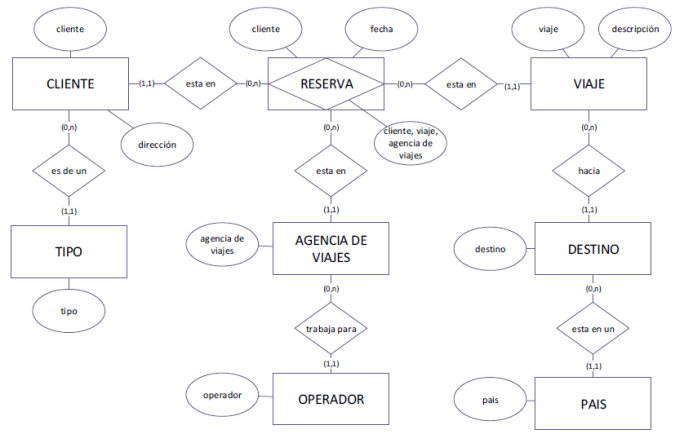
\includegraphics[width=17cm]{./Imagenes/2}
	\end{center}	

Por favor identifique el hecho de interés y construya el Modelo Dimensional y su respectivo esquema físico

DESARROLLO 
EJERCICIO 02

	\begin{center}
	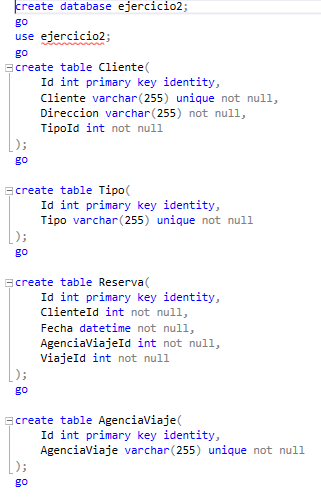
\includegraphics[width=17cm]{./Imagenes/21}
	\end{center}	

	\begin{center}
	
\includegraphics[width=17cm]{./Imagenes/22}
	\end{center}	

	\begin{center}
	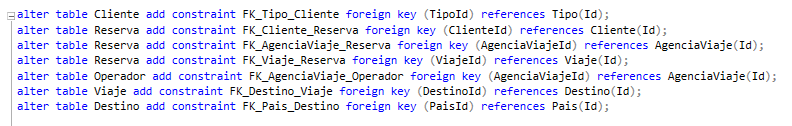
\includegraphics[width=17cm]{./Imagenes/23}
	\end{center}	

MODELO DIMENSION 02

	\begin{center}
	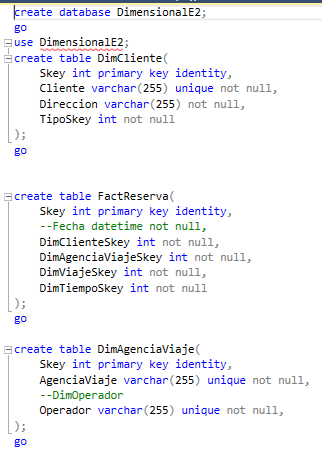
\includegraphics[width=17cm]{./Imagenes/24}
	\end{center}	

	\begin{center}
	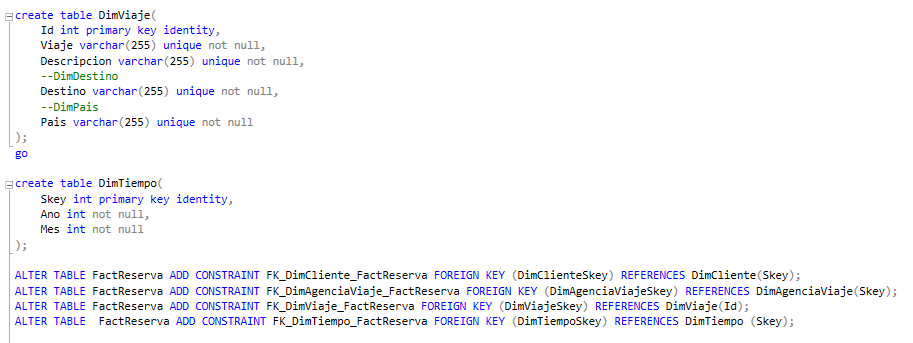
\includegraphics[width=17cm]{./Imagenes/25}
	\end{center}	